\documentclass[
	article,
	12pt,
	oneside,
	a4paper,
	english,
	brazil,
	sumario=tradicional
]{abntex2}

% Pacotes fundamentais
\usepackage{times}
\usepackage[T1]{fontenc}
\usepackage[utf8]{inputenc}
\usepackage{indentfirst}
\usepackage{color}
\usepackage{graphicx}
\usepackage{amsmath}
\usepackage{gensymb}
\usepackage{lscape}
\usepackage{pdflscape}
\usepackage[table,xcdraw]{xcolor}
\usepackage{float}
\usepackage{microtype}
\usepackage{multirow}
\usepackage[normalem]{ulem}
\usepackage{rotating}
\usepackage{booktabs}
\usepackage[alf,abnt-etal-cite=3,abnt-etal-list=0]{abntex2cite}
\usepackage{hyperref}
\usepackage{tabularx} % For tabularx environment
\usepackage{booktabs} % For \toprule, \midrule, and \bottomrule
\usepackage{caption} % For \captionsetup
\usepackage{makecell}
\usepackage{rotating}

\newcommand{\theforeigntitle}[1]{\def\@theforeigntitle{#1}}

% Configurações de aparência do PDF final
\definecolor{blue}{RGB}{41,5,195}
\hypersetup{
	pdftitle={Lista Extra de Econometria III},
	pdfauthor={Bruno Francisco Schaden},
	pdfsubject={Modelo de artigo científico com abnTeX2},
	pdfcreator={LaTeX with abnTeX2},
	pdfkeywords={abnt}{latex}{abntex}{abntex2}{artigo científico},
	colorlinks=true,
	linkcolor=blue,
	citecolor=blue,
	filecolor=magenta,
	urlcolor=blue,
	bookmarksdepth=4
}

% Configurações de margens
\setlrmarginsandblock{3cm}{2cm}{*}
\setulmarginsandblock{3cm}{2cm}{*}
\checkandfixthelayout

% Espaçamentos entre linhas e parágrafos
\setlength{\parindent}{1.5cm}
\setlength{\parskip}{0.2cm}
\OnehalfSpacing

% Informações de dados para CAPA e FOLHA DE ROSTO
\titulo{Lista Extra de Econometria III}
\autor{Bruno Francisco Schaden}
\local{Florianópolis}
\data{2024}

\begin{document}

\frenchspacing

% ELEMENTOS PRÉ-TEXTUAIS
\maketitle
\selectlanguage{english}

% Resumo em inglês
	\begin{resumoumacoluna}
	\noindent
	This list of Econometrics III exercises aims to replicate the results of the study by \cite{ENACHE2023102945} on the demand for in-app purchases in mobile applications. Using a difference-in-differences model to analyze exogenous price changes on the Apple platform, the paper, published in the International Journal of Industrial Organization, uses data from five word puzzle games across six European markets. The main objective is to estimate the price elasticity of demand for in-app purchases and understand how users responded to price changes. This list of exercises includes summarizing the main points and results of the article, explaining the identification hypotheses, detailing the difference-in-differences model, and reproducing the study's main figures and tables using Python.
	
	\textbf{Keywords:} In-app purchases. Mobile applications. Price elasticity of demand. Difference-in-differences. Exogenous price changes.
	
	\textbf{JEL Classification: }D12, L86, L13, L15, C23, L63
	\end{resumoumacoluna}

\newpage

\selectlanguage{brazil}
% Resumo em português
\renewcommand{\resumoname}{Resumo}
\begin{resumoumacoluna}
\begin{otherlanguage*}{brazil}
   \noindent 
   Esta lista de exercícios de Econometria III tem o objetivo de replicar os achados do estudo de \cite{ENACHE2023102945} sobre a demanda por compras no aplicativo em aplicativos móveis. Utilizando um modelo de diferença-em-diferenças para analisar mudanças exógenas de preços na plataforma Apple, o artigo, publicado no International Journal of Industrial Organization, usa dados de cinco jogos de quebra-cabeça de palavras em seis mercados europeus. O objetivo principal é estimar a elasticidade-preço da demanda por compras no aplicativo e entender como os usuários respondem às mudanças de preço. Esta lista de exercícios inclui resumir os pontos principais e os resultados do artigo, explicar a hipótese de identificação, detalhar o modelo de diferença-em-diferenças e reproduzir as principais figuras e tabelas do estudo utilizando Python. 
   
   \textbf{Palavras-chave}: Compras dentro do aplicativo. Aplicações Móveis. Elasticidade-preço da demanda. Diferença em diferenças. Mudanças exógenas de preços.
   
   \textbf{Classificação JEL:  }D12, L86, L13, L15, C23, L63
 \end{otherlanguage*}  
\end{resumoumacoluna}

\newpage


% ELEMENTOS TEXTUAIS
\textual

\section{Lista Extra - Replicação de estudo econométrico}

\subsection{Questão 1}
Faça um resumo do artigo, destacando os principais pontos do artigo e os resultados encontrados. (máximo 10 linhas)

\textbf{Resposta:} O artigo "Demand for in-app purchases in mobile apps—A difference-in-difference approach"  fala sobre como as mudanças nos preços de jogos freemium afetam os usuários em seis países europeus. Usando um método de diferença-em-diferenças, os autores analisaram ajustes de preços feitos pela Apple. Eles descobriram que quando os preços baixam, mais pessoas compram itens dentro dos aplicativos, com elasticidades variando entre -1 e -4. Por outro lado, assistir a vídeos para ganhar recompensas diminui. O número total de usuários não muda com a alteração dos preços. Esses resultados mostram que os usuários reagem bastante às mudanças nos preços e trocam entre gastar dinheiro ou tempo nos apps.

\subsection{Questão 2}
Explique a hipótese de identificação utilizada no artigo. É utilizada alguma variação exógena para identificação da elasticidade? (máximo 10 linhas)

\textbf{Resposta:} A hipótese do artigo se baseia nas mudanças de preços dos itens nos apps da Apple que foram feitas de forma independente pelos desenvolvedores. Em 2021, a Apple ajustou os preços em vários países, e essas mudanças foram vistas como fora do controle dos desenvolvedores. Isso permitiu que os autores usassem o método de diferença-em-diferenças, comparando como os usuários da Apple e do Google reagiram, já que os preços no Google não mudaram. Esse método ajudou a entender como a demanda reage aos preços, isolando o impacto das mudanças de preço da Apple.

\subsection{Questão 3}
O artigo utiliza um modelo de diferença-em-diferenças para estimar a elasticidade-preço da demanda por compras no aplicativo. Explique o que é um modelo de diferença-em-diferenças e como ele é utilizado no artigo. (máximo 10 linhas)

\textbf{Resposta:} Um modelo de diferença-em-diferenças é uma técnica que nos ajuda a entender os efeitos de uma mudança, comparando como as coisas mudaram em um grupo que foi afetado por uma intervenção com um grupo que não foi. No artigo, eles usam essa abordagem para ver como a demanda por compras em aplicativos muda com o preço. A intervenção foi o aumento de preços feito pela Apple em 2021. Os usuários da Apple são o grupo que foi afetado, enquanto os usuários do Google, que não tiveram mudança de preço, são o grupo de controle. Comparando as mudanças nas taxas de compra entre esses dois grupos antes e depois do aumento de preço, eles conseguem descobrir como a demanda reage ao preço.

\subsection{Questão 4}
Recrie a Fig.1 do artigo. Ela mostra “O número de usuários por dia do W1 em seis países europeus em torno de mudanças de preços na Apple. A figura mostra o número diário de usuários para janelas de 120 dias em ambos os lados de uma queda de preço na Apple em seis países europeus. O tempo de diminuição de preço é ilustrado por barras verticais e número de usuários por dia e plataforma são médias móveis de sete dias, normalizadas de modo que o número de usuários para 30 dias antes da mudança de preço definido como 1.” O número de usuários normalizados está na variável \texttt{userssmooth}.

\textbf{Resposta:} 

\begin{figure}[h!]
    \centering
    \caption{Número de usuários por dia do W1 em seis países europeus em torno de mudanças de preços na Apple.}
    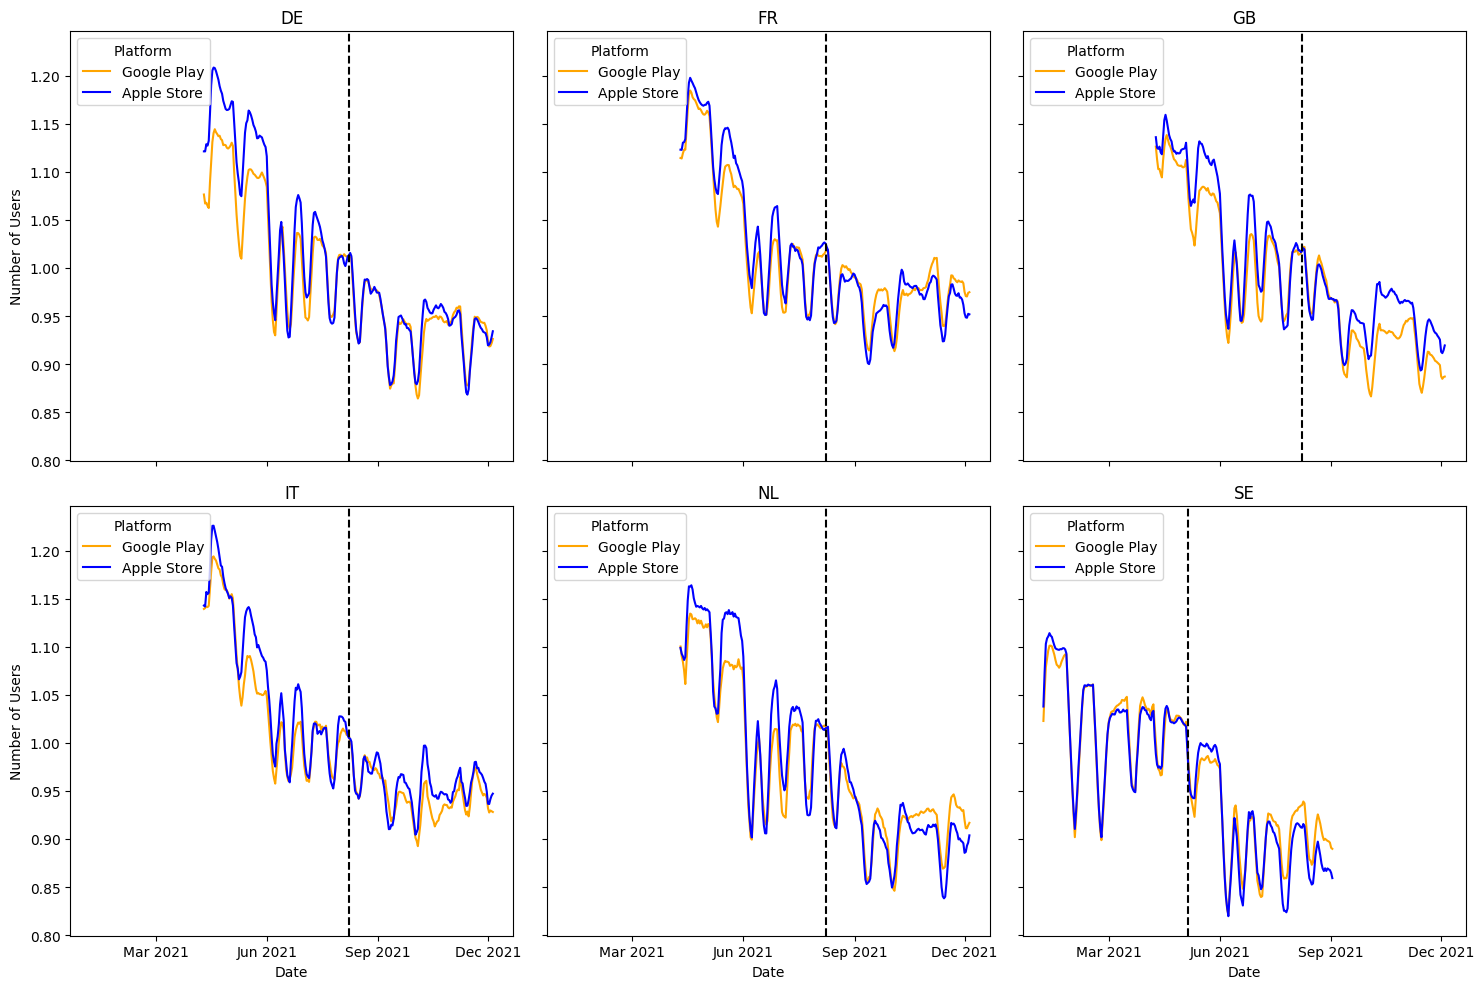
\includegraphics[width=0.8\textwidth]{Textuais/output.png}
    \fonte{Replicação - Elaborado pelos autores.}
\end{figure}

\newpage

\subsection{Questão 5}
Faça a tabela de estatísticas descritivas do conjunto de dados a semelhança da Tabela 1 do artigo. Entranto, além de incluir as médias dos jogos por país, inclua também o desvio padrão de cada uma das variáveis: \texttt{norm\_users}, \texttt{norm\_purch\_users}, e \texttt{norm\_videos}.

\textbf{Resposta:} 

\begin{sidewaystable}[htbp]
    \centering
    \renewcommand{\arraystretch}{1.1}
    \captionsetup{font=small}
    \caption{Estatísticas Descritivas dos Dados Normalizados}
    \label{tab:tabela_descritiva}
    \small % Ajusta o tamanho da fonte para 10 pontos
    \begin{tabularx}{\textwidth}{l*{14}{>{\raggedleft\arraybackslash}X}}
    \toprule
    Country & Game & Mean Norm Purch Users Google & Sd Norm Purch Users Google & Mean Norm Users Google & Sd Norm Users Google & Mean Norm Videos Google & Sd Norm Videos Google & Mean Norm Users Apple & Sd Norm Users Apple & Mean Norm Purch Users Apple & Sd Norm Purch Users Apple & Mean Norm Videos Apple & Sd Norm Videos Apple \\
    \midrule
    DE & W1 & 1.04 & 0.64 & 0.99 & 0.08 & 0.99 & 0.23 & 1.00 & 0.10 & 1.00 & 0.72 & 0.98 & 0.23 \\
    DE & W2 & 1.19 & 0.69 & 1.03 & 0.07 & 1.02 & 0.07 & 0.99 & 0.07 & 0.93 & 0.48 & 1.04 & 0.13 \\
    DE & W3 & 1.46 & 1.19 & 0.97 & 0.16 & 1.01 & 0.14 & 0.98 & 0.18 & 1.30 & 1.11 & 1.05 & 0.16 \\
    DE & W4 & 1.00 & 0.28 & 1.13 & 0.09 & 9.79 & 10.32 & 1.08 & 0.11 & 0.96 & 0.30 & 8.34 & 8.82 \\
    DE & W5 & 1.03 & 0.38 & 1.02 & 0.09 & 0.96 & 0.17 & 1.01 & 0.11 & 0.99 & 0.29 & 0.94 & 0.16 \\
    FR & W1 & 1.12 & 0.68 & 1.01 & 0.07 & 1.04 & 0.21 & 1.01 & 0.08 & 0.97 & 0.62 & 0.95 & 0.18 \\
    FR & W2 & 0.95 & 0.50 & 1.06 & 0.08 & 1.05 & 0.07 & 1.04 & 0.07 & 1.19 & 0.61 & 1.07 & 0.09 \\
    FR & W3 & 1.04 & 0.64 & 0.97 & 0.15 & 1.02 & 0.13 & 0.98 & 0.16 & 1.22 & 0.87 & 1.03 & 0.13 \\
    FR & W4 & 0.87 & 0.30 & 1.12 & 0.09 & 7.27 & 7.26 & 1.14 & 0.15 & 0.84 & 0.29 & 6.14 & 6.16 \\
    FR & W5 & 0.97 & 0.30 & 1.03 & 0.08 & 0.97 & 0.15 & 1.04 & 0.12 & 1.03 & 0.29 & 0.99 & 0.14 \\
    GB & W1 & 0.88 & 0.45 & 0.98 & 0.08 & 0.97 & 0.23 & 1.00 & 0.08 & 0.91 & 0.51 & 0.93 & 0.19 \\
    GB & W2 & 1.32 & 0.72 & 1.04 & 0.04 & 1.09 & 0.09 & 1.01 & 0.08 & 1.08 & 0.34 & 1.03 & 0.07 \\
    GB & W3 & 1.35 & 0.77 & 0.96 & 0.14 & 1.02 & 0.13 & 0.97 & 0.17 & 1.42 & 0.94 & 1.03 & 0.15 \\
    GB & W4 & 0.94 & 0.21 & 1.07 & 0.12 & 8.05 & 8.36 & 1.15 & 0.15 & 1.00 & 0.27 & 8.32 & 8.10 \\
    GB & W5 & 1.11 & 0.54 & 1.02 & 0.10 & 0.95 & 0.16 & 1.02 & 0.13 & 1.08 & 0.37 & 0.95 & 0.15 \\
    IT & W1 & 0.92 & 0.68 & 0.99 & 0.08 & 1.01 & 0.18 & 1.01 & 0.09 & 1.24 & 0.75 & 1.02 & 0.18 \\
    IT & W2 & 1.07 & 0.31 & 1.04 & 0.07 & 1.26 & 0.34 & 0.98 & 0.13 & 1.10 & 0.58 & 1.22 & 0.30 \\
    IT & W3 & 1.41 & 0.81 & 0.99 & 0.15 & 1.05 & 0.13 & 0.97 & 0.16 & 1.84 & 1.39 & 1.05 & 0.13 \\
    IT & W4 & 0.95 & 0.47 & 1.11 & 0.12 & 9.70 & 10.27 & 1.12 & 0.18 & 0.83 & 0.37 & 8.94 & 9.46 \\
    IT & W5 & 1.08 & 0.45 & 1.02 & 0.08 & 0.98 & 0.17 & 1.03 & 0.14 & 1.17 & 0.46 & 0.97 & 0.17 \\
    NL & W1 & 1.35 & 1.02 & 0.97 & 0.08 & 1.00 & 0.27 & 0.98 & 0.10 & 1.11 & 0.86 & 0.96 & 0.21 \\
    NL & W2 & NaN & NaN & 0.92 & 0.12 & 1.00 & 0.31 & 1.04 & 0.13 & 0.89 & 0.29 & 1.15 & 0.52 \\
    NL & W3 & 1.08 & 0.62 & 0.96 & 0.17 & 1.03 & 0.16 & 0.96 & 0.17 & 1.19 & 1.09 & 1.03 & 0.16 \\
    NL & W4 & 0.80 & 0.31 & 1.02 & 0.05 & 8.22 & 8.46 & 1.05 & 0.08 & 1.09 & 0.46 & 6.72 & 7.01 \\
    NL & W5 & 1.07 & 0.63 & 1.02 & 0.14 & 0.94 & 0.16 & 1.01 & 0.17 & 1.07 & 0.53 & 0.96 & 0.17 \\
    SE & W1 & 1.39 & 0.99 & 0.96 & 0.08 & 1.01 & 0.23 & 0.96 & 0.09 & 1.17 & 0.69 & 0.96 & 0.17 \\
    SE & W2 & 0.94 & 0.62 & 0.98 & 0.10 & 1.03 & 0.23 & 1.04 & 0.15 & 1.29 & 0.58 & 0.95 & 0.14 \\
    SE & W3 & 1.10 & 0.82 & 0.96 & 0.16 & 1.01 & 0.15 & 0.96 & 0.18 & 1.12 & 0.64 & 0.99 & 0.16 \\
    SE & W4 & 1.13 & 0.33 & 1.05 & 0.20 & 1.70 & 3.00 & 0.91 & 0.07 & 0.86 & 0.34 & 1.33 & 1.80 \\
    SE & W5 & 0.83 & 0.39 & 0.98 & 0.16 & 1.07 & 0.27 & 0.96 & 0.12 & 0.98 & 0.38 & 1.02 & 0.26 \\
    \bottomrule
    \end{tabularx}
\fonte{Elaborado pelos autores.}
\end{sidewaystable}

\newpage

\subsection{Questão 6}
Recrie a Fig. 7 do artigo. Ela mostra a “Taxa de conversão por dia em W1 em seis países europeus em torno de mudanças de preços na Apple. A figura mostra o número diário de compras no aplicativo / número de usuários para janelas de 120 dias em ambos os lados de uma mudança de preços na Apple em seis países europeus. O momento das mudanças de preço é ilustrado por barras verticais e o número de usuários por dia e plataforma são médias móveis de sete dias, normalizadas para que o número diário de compras no aplicativo / número de usuários para 30 dias antes da mudança de preço seja definido como 1.” A taxa de conversão normalizada está na variável \texttt{purchsmooth}.

\textbf{Resposta:} 

\begin{figure}[h!]
    \centering
    \caption{Taxa de conversão por dia no W1 em seis países europeus em torno das alterações de preços na Apple.}
    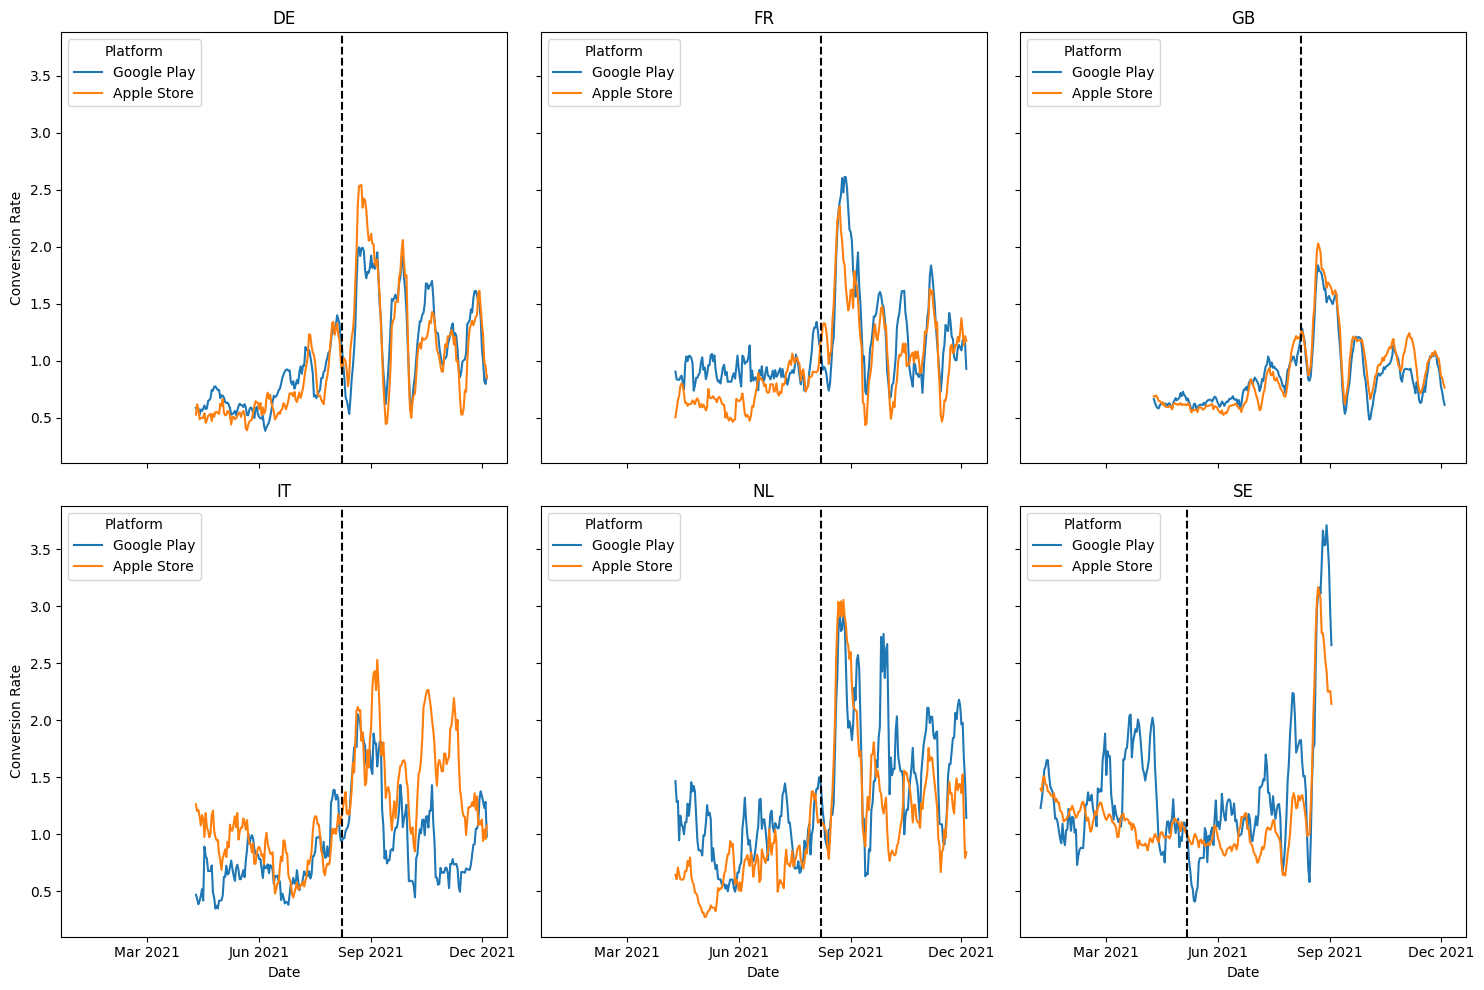
\includegraphics[width=0.8\textwidth]{Textuais/output fig7.png}
    \fonte{Replicação - Elaborado pelos autores.}
\end{figure}

\newpage

\subsection{Questão 7}
Recrie a Tabela 4 painel A do artigo. Você deve inferir quais são as variáveis utilizadas na regressão dos autores, entretanto, a interação entre país e jogo é representada pela variável \texttt{cgn}. Além disso, os dados não nos fornecem a variação de preços ponderada, portanto não conseguimos computar a linha \texttt{Price change}. Se tomarem aqueles valores das variações de preço como dados, calculem a linha \texttt{Elasticity}.

\textbf{Resposta:} 

\begin{table}[htbp]
    \centering
    \renewcommand{\arraystretch}{1.1}
    \captionsetup{font=small}
    \caption{Estimativas de DID, efeito do tratamento das alterações de preços na taxa de conversão.}
    \label{tab:tabela_resultados}
    \small % Ajusta o tamanho da fonte para 10 pontos
    \begin{tabularx}{\textwidth}{l*{6}{>{\raggedleft\arraybackslash}X}}
    \toprule
     & Full Sample & W1 & W2 & W3 & W4 & W5 \\
    \midrule
    Post x Apple & 0.158*** & 0.169*** & 0.161*** & -0.073 & 0.381*** & 0.104*** \\
    Std. Error & (0.019) & (0.034) & (0.046) & (0.049) & (0.026) & (0.028) \\
    Num. Obs. & 12655.00 & 2772.00 & 2069.00 & 2077.00 & 2877.00 & 2860.00 \\
    R² Adj. & 0.106 & 0.564 & 0.109 & 0.265 & 0.216 & 0.259 \\
    Price Change & -0.105 & -0.114 & -0.102 & -0.126 & -0.092 & -0.097 \\
    Elasticity & -1.500 & -1.480 & -1.574 & 0.576 & -4.144 & -1.070 \\
    \bottomrule
    \end{tabularx}
    \caption{Níveis de significância: $p < 0.1$, * $p < 0.05$, ** $p < 0.01$, *** $p < 0.001$. \newline
    Os erros padrão robustos (HC1) foram utilizados para \texttt{cov\_type}, conforme indicado na legenda da tabela original.}

\fonte{Elaborado pelos autores.}
\end{table}


\postextual
% ELEMENTOS PÓS-TEXTUAIS
\renewcommand{\refname}{Referências}
\bibliographystyle{abntex2-alf}
\bibliography{Referencias}

%
% ----------------------------------------------------------
% Apêndices
% ----------------------------------------------------------

% ---
% Inicia os apêndices
% ---
\begin{apendicesenv}

\end{apendicesenv}

\end{document}
